\section{SMAWK}
\label{SMAWK}

%----------------------------------------------------------------------------------------

Nesta seção discutiremos o algoritmo SMAWK. Ele é conhecido pela sua aplicação no problema de encontrar o vértice mais distante de cada vértice num poígono convexo em tempo linear~\cite{Aggarwal:1987}. Ao final desta seção serão explicadas esta e outras aplicações deste algoritmo.  

Dada uma matriz $A \in \B{Q}^{n \times m}$, listamos os casos de uso deste algoritmo:
\begin{itemize}
    \item Se $A$ é totalmente monótona convexa ou côncava nas linhas podemos encontrar os índices de mínimos e máximos das linhas em tempo $\Cl{O}(n + m)$ e
    \item se $A$ é totalmente monótona convexa ou côncava nas colunas podemos encontrar os índices de mínimos e máximos das colunas em tempo $\Cl{O}(n + m)$.
\end{itemize}

Apresentaremos o caso onde $A$ é totalmente monótona convexa nas linhas e estamos interessados nos índices de mínimos. Na Subseção~\ref{SMAWK_Generalizacoes} explicamos como reduzir os problemas elencados para este caso.
%----------------------------------------------------------------------------------------

\subsection{Técnica Primordial}
Para facilitar a compreensão do algoritmo SMAWK, iremos apresentar uma técnica parecida com a Divisão e Conquista apresentada na Seção~\ref{DivisaoEConquista} e mostrar uma otimização desta técnica que leva ao algoritmo SMAWK.

Dada uma matriz~$A \in \B{Q}^{n \times m}$ totalmente monótona convexa por linhas, queremos encontrar o menor índice de mínimo de cada uma das linhas de~$A$. Se para uma dada linha~$i$ onde~$i > 0$ e~$i < n$ conhecermos os índices~$l$ e~$r$ de mínimos das linhas~$i-1$ e~$i+1$, respectivamente, já que~$A$ tem os índices de mínimos das linhas crescente (por ser totalmente monótona) basta buscar o índice de mínimo da linha~$i$ no intervalo entre~$l$ e~$r$ (inclusive). Além disso, se~$i$ é a primeira linha da matriz podemos considerar~$l = 1$ ou se~$i$ é a última linha da matriz podemos considerar~$r = n$ sem perder a validade do fato de que basta buscar entre~$l$ e~$r$.  

Após realizar as observações acima note que, já que~$A$ é totalmente monótona, remover qualquer linha de~$A$ mantém a total monotonicidade e não altera o índice de mínimo de outra linha. Com esta observação, concluímos que podemos remover todas as linhas pares da matriz, resolver o problema recursivamente para a matriz resultante e utilizar este resultado para calcular os índices de interessa para as linhas pares da matriz.  

Com uma análise similar à realizada para a técnica da Divisão e Conquista é fácil concluir que uma implementação desta técnica que consiga remover as linhas pares da matriz (e adicionar elas de volta) em tempo~$\Cl{O}(1)$ resolve o problema em tempo~$\Cl{O}((n+m)\lg(n))$, assim como a técnica da divisão e conquista.  
%----------------------------------------------------------------------------------------

\subsection{Reduce}
Queremos agilizar a técnica apresentada acima. Para isso, vamos adicionar uma nova hipótese. Vamos supor que a matriz~$A$ é quadrada, ou seja,~$n = m$. Lembre que a cada passo, removemos as~$\floor{n/2}$ linhas pares da matriz gerando uma nova matriz $A'$, resolvemos o problema recursivamente para~$A'$ e usamos a solução de~$A'$ para resolver para as linhas restantes de~$A$. O problema é que quando removemos linhas da nossa~$A$, ela deixa de ser quadrada e passa a ser uma matriz com mais colunas do que linhas, isto é,~$m \geq n$. Chamamos de ótimas as células da matriz que são mínimo de alguma linha e as colunas que contém o índice de mínimo de pelo menos uma linha. Note que uma matriz contém no máximo~$n$ colunas ótimas, pois cada linha faz com que exatamente uma célula seja ótima. Queremos remover colunas não ótimas de uma matriz~$A$ com mais colunas do que linhas fazendo com que~$A$ se torne quadrada.  

Vamos desenvolver o algoritmo \textsc{Reduce} a partir de um índice de linha~$k \leq n$ e de uma invariante: Toda célula com índices de linha menor do que~$k$ e coluna menor ou igual a~$k$ não é ótima. Se o índice~$k$ representa uma coluna, a invariante nos diz que todas as células acima da diagonal principal que estão nesta coluna ou à esquerda dela são não ótimas. A Figura~\ref{figure:Reduce1} representa, em azul, a célula de índice~$k,k$ e, em preto, as células que, segundo a invariante, são não ótimas.

\begin{figure}[h]
    \centering
    % === Based On ===
% Geometric representation of the sum 1/4 + 1/16 + 1/64 + 1/256 + ...
% Author: Jimi Oke
% ================

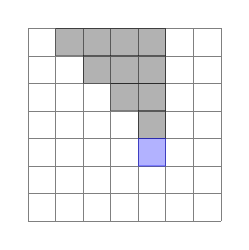
\begin{tikzpicture}[scale=.35]\footnotesize
 \pgfmathsetmacro{\xone}{0}
 \pgfmathsetmacro{\xtwo}{7}
 \pgfmathsetmacro{\yone}{0}
 \pgfmathsetmacro{\ytwo}{7}

\begin{scope}<+->;
% grid
  \draw[step=1cm,gray,very thin] (\xone,\yone) grid (\xtwo,\ytwo);
\end{scope}

% function
\begin{scope}[thin,black,opacity=.3]
  \filldraw (1,7) rectangle (5,6);
  \filldraw (2,6) rectangle (5,5);
  \filldraw (3,5) rectangle (5,4);
  \filldraw (4,4) rectangle (5,3);
  \filldraw[blue] (4,3) rectangle (5,2);
\end{scope}

\end{tikzpicture}

    \caption{Invariante do \textsc{Reduce}.} \label{figure:Reduce1}
\end{figure}

Primeiramente, se~$k \leq n$ e a entrada~$A[k][k+1]$ não existir na matriz, ela não tem mais colunas do que linhas e não precisamos aplicar o \textsc{Reduce}. Se~$A[k][k] > A[k][k+1]$, toda a coluna~$k$ é não ótima e pode ser removida. Para demonstrar isso, escolhemos um índice de linha~$i$ qualquer e mostramos que $A[i][k]$ é não ótimo. Se~$i < k$ o fato segue da invariante e se~$i = k$ também é verdade pois $A[k][k+1]$ pertence à mesma linha e tem valor estritamente menor. Agora, se~$i > k$, pela definição de total monotonicidade temos~$A[i][k] \leq A[i][k+1]$ implica $A[k][k] \leq A[k][k+1]$, basta aplicar a contrapositiva nesta afirmação e observar que~$A[i][k] > A[i][k+1]$, portanto~$A[i][k]$ também é não ótima. Note que se removermos a coluna~$k$ da matriz e não alterarmos o índice~$k$, a invariante não será mantida, basta subtrair~$1$ de~$k$ para manter a invariante.

Agora, se~$A[k][k] \leq A[k][k+1]$, vamos mostrar que todos os elementos da coluna $k+1$ que estão em uma linha maior ou igual à $k$-ésima são não ótimos.

%----------------------------------------------------------------------------------------

\subsection{SMAWK}
%----------------------------------------------------------------------------------------

\subsection{Análise}
%----------------------------------------------------------------------------------------

\subsection{Implementação}
%----------------------------------------------------------------------------------------

\subsection{Generalizações} \label{SMAWK_Generalizacoes}
